\documentclass[12pt, a4paper]{article}

\usepackage{amsmath, amsfonts, amsthm}
\usepackage{graphicx, subfigure}      
\usepackage{cite, xspace, fullpage}   
\usepackage{color}                    
\usepackage{setspace}
\usepackage{url}

\parskip 6pt
\parindent 0pt

\begin{document}

\title{WhatsApp based Symptom Tracker (WaSyT)}


\author{Fadi Zaraket, \\
  Department of Electrical and Computer Engineering, \\ 
  American University of Beirut}

\date{}
%\nodate
%\date{\today}

\maketitle

\thispagestyle{empty}

\bigskip \bigskip
\hrule
\bigskip \bigskip



% \underline{Subject:} Proposal, Spring 2019-2020.

% \underline{Investigator:} Prof. Fadi Zaraket, Electrical and Computer
% Engineering, MSFEA, AUB

% \underline{Title:} {\bf Limited Internet Symptom Tracker}

% \underline{Date:} April 2, 2020

% \bigskip \bigskip
% \hrule
% \bigskip \bigskip


Public health policies across the globe may have differed from one
place to another, but all agreed on the need to detect early Covid-19
cases. Possibly due to limited resources and technologies, testing has
been limited in some countries to patients exhibiting symptoms and in
many cases multiple symptoms. Needless to point out the large strain
that the situation is imposing on national health care systems and
workers even in those in most developed countries, feeding into the
difficulties of identifying and tracking possible cases.

On a parallel front, epidemiologists have been trying to identify
common symptoms, their order of appearance, percentages of occurrences
and various statistics related to that matter.

Both objectives created the need for large data collection from
residents of a --possibly large-- geographic area outside the common
practices of visiting a health care professional for diagnosis and
follow up. Such data may naturally help researchers understand better
how fast the virus is spreading, identify hot spots, provide
scientists individual recommendations and even possibly alert
residents. A symptom tracking mobile app has been launched for example
in the UK through an effort led by King's College allowing any user to
self-report possibly on a daily basis on their symptoms or lack of.

The premise of a large-scale mechanism where individuals self-report
is naturally dependent on a large-scale connectivity of
residents. Within the Lebanese society three observations can be made:
\begin{itemize}
\item A substantial portion of the population has limited wireless
  internet connection, whereby WhatsApp packages are common and only
  WhatsApp is available.
\item A substantial portion is not ``device savvy'' and installing an
  app is often done through a store or an acquaintances. One may argue
  that this group of people should be especially targeted.
\item Maybe to a lesser extent, a portion of potential users are not
  multi-lingual and only versed in Arabic.
\end{itemize}

% Phone Ogero
% Webbased

\subsection*{Objectives}

The scope of this work targets primarily bridging the gap of limited
wireless connectivity by providing an alternative that serves directly
addressing the two additional shortcomings listed above.

At a high level, the project dedicates WhatsApp enabled phone numbers
for receiving messages possibly containing symptoms. Similarly to the
WHO information WhatsApp robot, our robots extract from both text and
audio messages symptoms and save them into a database. The database
entries will relate users, their locations and symptoms across time.

Sample messages will look as in Figure~\ref{fig:sample}.

\begin{figure}[!htb]
  \begin{center}
    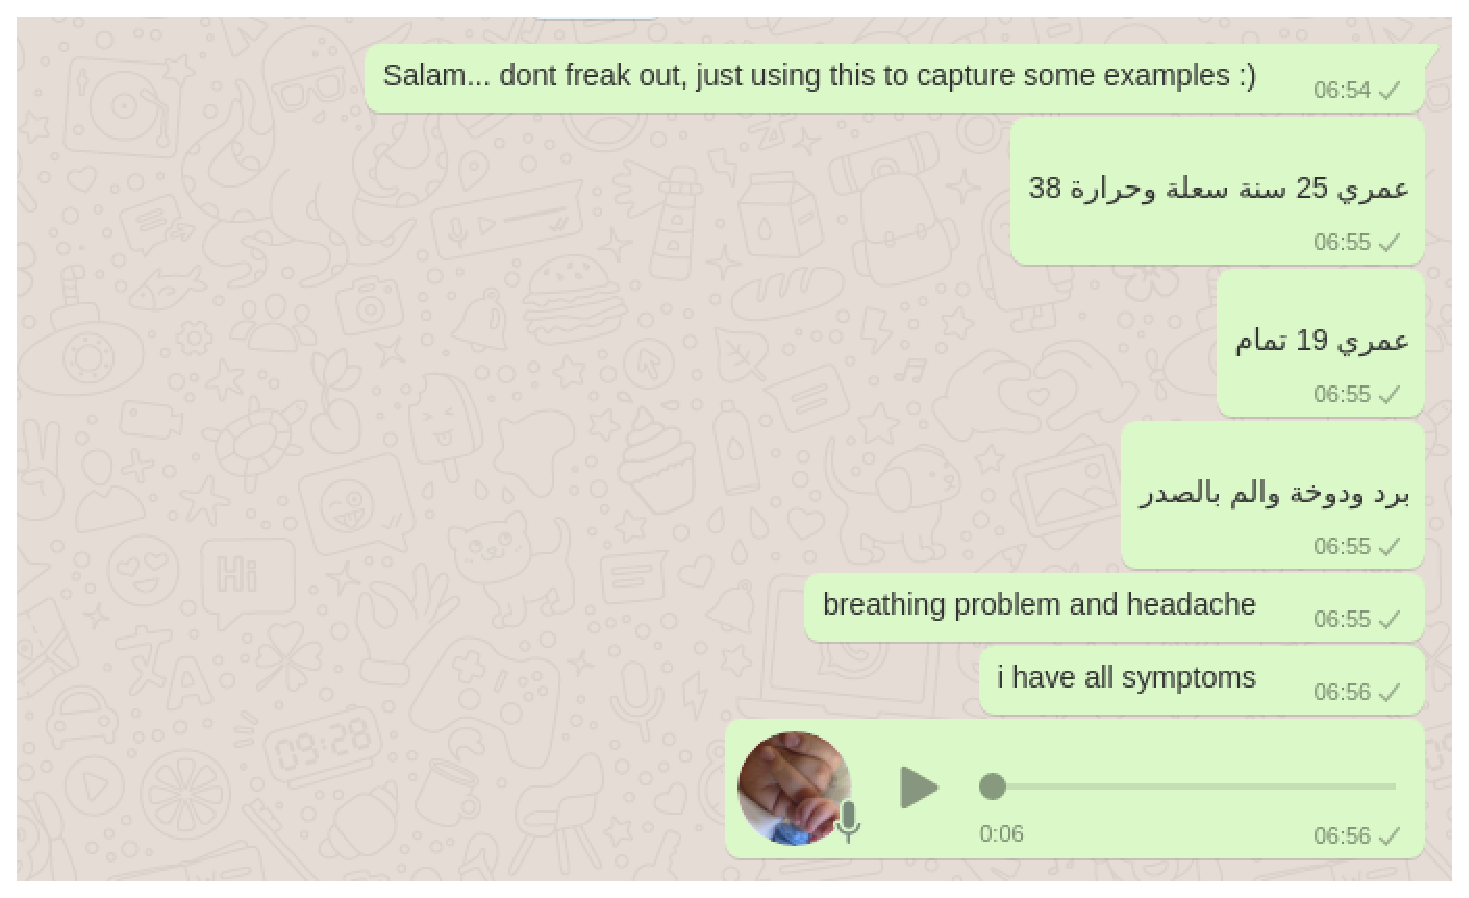
\includegraphics[width = 13cm]{examples.eps}
    \caption{Sample messages.\label{fig:sample}}
  \end{center}
\end{figure}


\subsubsection*{Downstream}

With the data available, multiple data analytics tasks may be
performed including statistics collection, modeling, analysis and
possibly recommendations on interventions. These data-based tasks are
not considered as a direct objective of this project at this time.



\subsection*{How does it work}

The teams member investigated multiple solutions for various aspects
of the project:

\begin{itemize}
\item WhatsApp-related infrastructure:

  Two alternatives were implemented to recover messages whether text,
  audio or location.
  \begin{itemize}
  \item \underline{WhatsApp business API}

    % Partnership with WhatsApp
    
    A paid service for regional service providers may be used to
    ``acquire'' the received messages on the dedicated WhatsApp numbers.
    
    In collaboration with \url{CM.com} a trial was successfully conducted
    whereby a received message --whether text, audio or location-- is
    acquired on a dedicated server.
    
    \underline{Notes:} Whereas this solution has been developed, it is
    noted that it is a paid service and its deployment requires an
    estimate of 2,500 USD  is required per 500,000 Messages subject to renewal
      and negotiation.
    
  \item \underline{Browser extensions over {\em web.whatsapp.com\/}}
        
    The team developed a ``chrome'' extension that can be installed
    that allows recovering the message received.

    In broad terms, through the web portal of WhatsApp, JavaScript
    listeners download the received messages --whether text, audio or
    location-- and store them for further processing.
      
  \end{itemize}

\item Text message decoding:

  Members of the team 
 %   and with the collaboration of ????? 
    used Natural
  Language Processing to decode text messages and identify whether and
  what symptom ``keywords'' are present. The results are logged and
  stored in an appropriately designed database.

\item Audio message decoding:

  When it comes to Speech Recognition, with the collaboration of RDI-ai
  voice messages are decoded, transformed into text and the same
  solution presented above is then used.
  The RDI solution is also a paid licensed solution. 
  The team is working on an alternative solution based on the John  
  Hopken's open source Kaldi speech recognition system and have 
    obtained an Arabc transcribed data set from QCRI for that. 
    The team also collected its own audio dataset of 500 sentences 
    including symptoms to boost the speech recognition models.

\end{itemize}


\subsection*{Where does it stand in the spectrum}

Multiple initiatives with various degrees of success have been
undertaken globally. We note here a few.

\begin{itemize}
\item[$\bullet$] King’s College London and Guy’s and St Thomas’
  Biomedical Research Center~\cite{Kings}.

  Through this application users communicate daily their symptoms. As
  of April 6, 2020 the app has been installed by more than 500,000
  users.

\item[$\bullet$] The WHO COVID-19 WhatsApp Robot.

  The WHO and WhatsApp created a chatbot to share reliable coronavirus
  info~\cite{WHOWA}. On a larger scale, ``The WhatsApp Coronavirus
  Information Hub'' is in partnership with the United Nations
  Development Programme, the World Health Organization and
  UNICEF~\cite{WHOWAI}.
  
\item[$\bullet$] Apple's COVID-19 app and website (based on CDC
  guidance)~\cite{Apple}.

  The application is intended to be a screening tool and help people
  stay informed. Users answer a series of questions around risk
  factors, recent exposure and symptoms and they receive in return CDC
  recommendations on possible next steps.

\item[$\bullet$] India's ``{\em MyGov Corona
    Helpdesk\/}''~\cite{India}.

  With the primary objective of fighting rumors and education, this
  WhatsApp robot provides authoritative answers to coronavirus queries.
  
  
\item[$\bullet$] The Lebanese Ministry of Public Health symptom
  checker~\cite{MoPH}.
  
\item[$\bullet$] AUBMC added symptom checker within its AUBHealth
  Mobile App.

\end{itemize}


\subsection*{Final Notes}

Since Lebanon is not a singular case when it comes to WhatsApp
penetration rate vs cellular internet penetration rate, the solutions
provided here are naturally applicable in all such environments
especially the Arabic-speaking ones.  If and wherever adopted, a
tutorial and promotion campaign is necessary to maximize the reaped
potential benefits of this tool.


The team was lead by ECE Prof. Fadi Zaraket and Prof. Ibrahim Abou-Faycal 
and consisted of MSFEA's ECE students:
\begin{itemize}
%\item Hadi Ayache   
\item Nourhane Abdel-Samad
\item Christophe Haddad 
\item Ali Al-Akbar Haidoura 
\item Hadi Kotaich
\item Ayham Olleik
%\item Abdallah Dandashli
\end{itemize}

The source code for the various solutions presented above are made
available by the team on \url{https://github.com/HadiKotaich/SocialMediaSymptomTracker}


% \bigskip \bigskip \bigskip

% ~\hspace{6cm}{Ibrahim Abou-Faycal

% ~\hspace{6cm}Prof. of Elec. and Comp. Eng.}

\bibliographystyle{unsrt}
\bibliography{SymTr}

\end{document}

